\documentclass[../mainfile.tex]{subfiles}
\begin{document}
\section{Differenzengleichung}
\subsection*{Beispiel:}
Ein Wald wächst jährlichg um 12\% und hat momentan 12 000 Bäume. Jährlich werden 500 Bäume geschlägert.\\
$B_0 = 12000\\
B_1=12000*1,12-500\\
B_2=B_1*1,12-500=1200*1,12^2-500*1,12-500\\
...\\
$
Wird angewandt bei beschänktem und logistischem Wachstum.\\
\begin{figure}[h]
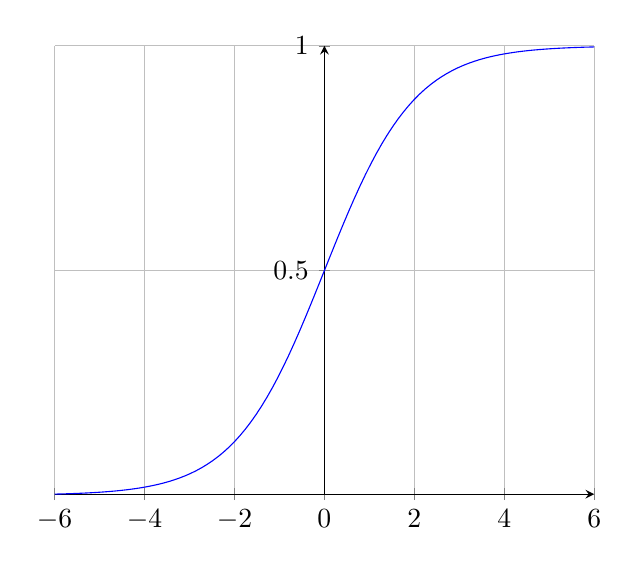
\begin{tikzpicture}
    \begin{axis}%
    [
        grid=major,     
        xmin=-6,
        xmax=6,
        axis x line=bottom,
        ytick={0,.5,1},
        ymax=1,
        axis y line=middle,
    ]
        \addplot%
        [
            blue,%
            mark=none,
            samples=100,
            domain=-6:6,
        ]
        (x,{1/(1+exp(-x))});
    \end{axis}
\end{tikzpicture}

\end{figure}
\begin{figure}[h]
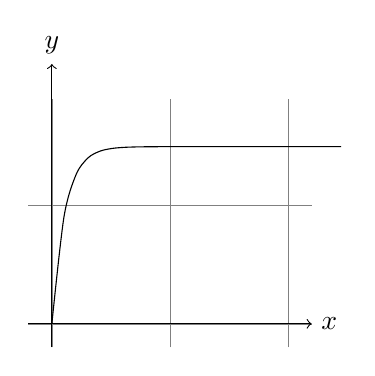
\begin{tikzpicture}[scale=0.15]
	\draw[very thin,color=gray,step=10.0] (-2,-2.0) grid (22.0,19.0);
    \draw[->] (-2,0) -- (22,0) node[right] {$x$}; 
    \draw[->] (0,-2.0) -- (0,22.0) node[above] {$y$};
	\draw[scale=0.5,domain=0:49,smooth,variable=\x] plot ({\x},{30-30*exp(-0.45*\x)});
\end{tikzpicture}
\end{figure}

\end{document}